\section{Results}
\label{sec:results}

\paragraph{Ground-truth reliability is the binding constraint.}
Of the \sensNPackages{} eligible packages, only \nPackages{} (\reliableFraction{}) have a
statistically reliable within-package winner (Figure~\ref{fig:reliability}).

\begin{figure}[t]
  \centering
  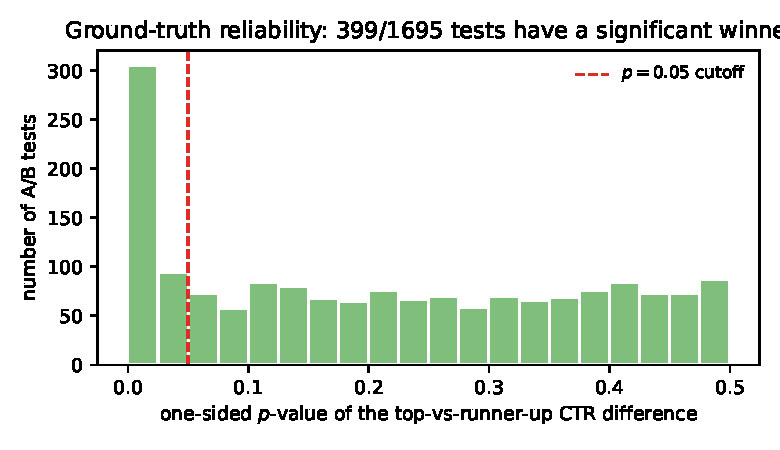
\includegraphics[width=0.92\linewidth]{figures/reliability.pdf}
  \caption{Distribution of the one-sided $p$-value for the top-vs-runner-up CTR difference across
  the eligible A/B tests. Only the tests to the left of the dashed cutoff have a statistically
  reliable winner; the rest cannot be predicted by construction.}
  \label{fig:reliability}
\end{figure} In the remainder the real click-through difference is indistinguishable
from noise, so no predictor can recover the ordering by construction. The primary analysis is
therefore restricted to the \nPackages{} reliable packages.

\paragraph{Personas vs.\ a no-persona baseline (RQ1).}
Table~\ref{tab:validity} reports within-package ranking agreement (Section~\ref{sec:framework})
on the reliable packages for both methods. The headline result is that \emph{persona conditioning
hurts}. The no-persona zero-shot baseline ranks variants well---Kendall $\tau=\baseTau{}$ (95\% CI
[\baseTauCILow{}, \baseTauCIHigh{}]), a medium effect by Cohen's
conventions~\citep{cohen1988power}, with top-1 accuracy \baseTopOne{} (95\% CI
[\baseTopOneCILow{}, \baseTopOneCIHigh{}]) against a random baseline of \randomTopOne{}. The
ten-persona panel is far weaker: $\tau=\kendallTau{}$ (95\% CI
[\kendallTauCILow{}, \kendallTauCIHigh{}]) and top-1 \topOneAcc{}, with confidence intervals that
do not overlap the baseline's on any metric (Figure~\ref{fig:comparison}). Persona conditioning
thus does not merely fail to help---it actively degrades a usable signal that the base model
already has.

\begin{figure}[t]
  \centering
  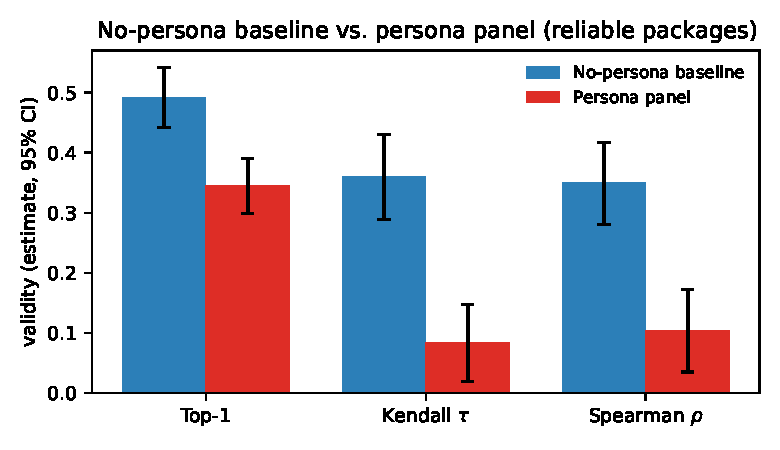
\includegraphics[width=0.92\linewidth]{figures/comparison.pdf}
  \caption{Headline result: the no-persona baseline outperforms the persona panel on every
  metric, with non-overlapping 95\% bootstrap CIs, on the reliable-winner packages.}
  \label{fig:comparison}
\end{figure}

\paragraph{The persona panel in isolation.}
Considered on its own, the panel's predictive validity is weak but statistically significant
($\tau$ and $\rho$ CIs exclude zero), at or below Cohen's small-effect threshold. Its top-1 CI
includes the random baseline, so it does not reliably pick the single best variant; it is, if
anything, slightly better at flagging the \emph{worst} variant (\bottomOneAcc{}) than the best
(\topOneAcc{}), detecting clearly weak copy more readily than winners.

% AUTO-GENERATED by scripts/generate_validity_table.py — DO NOT EDIT BY HAND.
\begin{table*}[t]
  \centering
  \caption{Headline result: a no-persona zero-shot ranker vs.\ the persona panel on the reliable-winner packages ($n=399$). The no-persona baseline is substantially better on every metric (non-overlapping CIs). Random top-1 baseline 30.4\%. 95\% bootstrap CIs.}
  \label{tab:validity}
  \small
  \begin{tabular}{lccc}
    \toprule
    Method & Top-1 [95\% CI] & Kendall $\tau$ [95\% CI] & Spearman $\rho$ [95\% CI] \\
    \midrule
    No-persona baseline & 49.2\% [44.2, 54.3] & 0.361 [0.289, 0.430] & 0.350 [0.281, 0.417] \\
    Persona panel & 34.6\% [29.8, 39.1] & 0.084 [0.020, 0.147] & 0.104 [0.035, 0.172] \\
    \bottomrule
  \end{tabular}
\end{table*}


\paragraph{Sensitivity analysis.}
Including all \sensNPackages{} predicted packages (i.e.\ without the reliability filter) the
effect is weaker but remains significant ($\tau=\sensKendallTau{}$, 95\% CI
[\sensKendallTauCILow{}, \sensKendallTauCIHigh{}]; $\rho=\sensSpearmanRho{}$), as expected when
noisy-label packages are added.

\paragraph{Does validity track signal strength? (RQ2).}
Across \hThreeN{} packages spanning the full range of ground-truth signal strength, stronger
real effects are associated with slightly higher top-1 success (Spearman $\hThreeTopOne{}$, 95\%
CI [\hThreeTopOneCILow{}, \hThreeTopOneCIHigh{}]), while the association with the full
rank-correlation is null. The simulator captures a small amount of signal that surfaces mainly
when the real effect is large.

\paragraph{Replication across datasets and a different domain (RQ3).}
The finding replicates. Table~\ref{tab:replication} repeats the comparison on three independent
Upworthy splits and on a different-domain, more-recent dataset (MIND news, 2019). On all three
Upworthy A/B splits the no-persona baseline beats the persona panel by a large, consistent
margin (Kendall $\tau$ gap between \repGapMin{} and \repGapMax{}); the powered confirmatory split
($n=\confNPackages{}$) gives the cleanest contrast ($\tau=\confBaselineTau{}$ baseline vs.\
$\confPersonaTau{}$ persona). On MIND---where ``packages'' compare \emph{different} articles
within a topic rather than headline variants of one story---the direction is the same but the gap
is small ($\mindGap{}$), as expected when persona-relevant variance is lower. A boundary case is
Reddit title reposts (same image, different titles): there upvotes are dominated by posting time
and visibility rather than the title, \emph{neither} method predicts the outcome (both
$\tau\approx0$), and the gap vanishes---the baseline's advantage appears only where the outcome is
actually predictable from the copy. We also report a
decision-relevant metric, the fraction of achievable CTR lift captured by the top-1 pick: the
baseline captures more than the panel in every dataset (Table~\ref{tab:replication}).
% AUTO-GENERATED by scripts/generate_replication_table.py — DO NOT EDIT BY HAND.
\begin{table*}[t]
  \centering
  \caption{Replication across three independent Upworthy splits and two further platforms/domains (MIND news, 2019; Reddit title reposts, 2008--12). The no-persona baseline beats or matches the persona panel everywhere; the advantage is large on controlled copy A/B tests, small on cross-article news, and vanishes on Reddit where upvotes are not title-predictable (both $\tau\approx0$). Lift = fraction of achievable CTR lift captured by the top-1 pick (persona/baseline). Kendall $\tau$ on significant-winner packages. For cross-dataset comparability all rows use a single draw per persona; the exploratory split's multi-draw primary estimate is in Table~\ref{tab:validity}.}
  \label{tab:replication}
  \small
  \begin{tabular}{lccccc}
    \toprule
    Dataset & $n$ & Persona $\tau$ & Baseline $\tau$ & Gap & Lift p/b \\
    \midrule
    Upworthy exploratory (2013--15) & 399 & 0.079 & 0.361 & $+0.282$ & 0.45/0.58 \\
    Upworthy holdout (2013--15) & 402 & 0.100 & 0.398 & $+0.298$ & 0.48/0.56 \\
    Upworthy confirmatory (2013--15) & 1866 & 0.070 & 0.393 & $+0.323$ & 0.44/0.55 \\
    MIND news (2019) & 74 & 0.177 & 0.214 & $+0.038$ & 0.47/0.51 \\
    Reddit titles (2008--12) & 600 & -0.009 & -0.026 & $-0.017$ & 0.45/0.33 \\
    \bottomrule
  \end{tabular}
\end{table*}


\paragraph{Robustness: seed and model (RQ3).}
On a 100-package subset re-run under three seeds, top-1 accuracy is highly stable
(SD $=\stabTopOneSD{}$) while the rank coefficient varies by SD $=\stabTauSD{}$ in $\tau$---
non-trivial relative to the effect size, which is why the primary estimate averages multiple
draws. The persona-vs-baseline gap is also consistent across model tiers: on all three
\texttt{gemini} models the no-persona baseline beats the persona panel
(Table~\ref{tab:cross_model_gap}), so ``personas hurt'' is not an artefact of a single model. Nor
is it a prompt artefact: a third-person persona framing and a reworded baseline leave both sides
essentially unchanged---the persona panel stays weak under either framing and the baseline stays
strong---so the gap is not driven by the specific wording of either prompt.

\paragraph{The reported gap is a conservative lower bound.}
The baseline is \emph{less} granular than the panel: on \baseTieRate{} of packages all its
variants receive an identical score and the top-1 pick is a tie, broken arbitrarily. This barely
moves the metric (baseline top-1 \baseTopOne{} under arbitrary tie-breaking vs.\ \baseTopOneFair{}
under fair $1/k$ tie credit), and on the non-tied packages the baseline reaches
\baseTopOneNonDegen{}. Because ties drag the baseline's score down,
the persona-vs-baseline gap we report is, if anything, an \emph{under}-estimate of the baseline's
true advantage.

\paragraph{Robustness: aggregation rule (RQ3).}
The primary estimate pools the panel with an arithmetic mean; to rule out that the result is an
artefact of this one choice, we re-aggregate the \emph{same} per-persona observations under six
rules (Table~\ref{tab:h5agg}). None recovers baseline validity---every persona configuration's
$\tau$ confidence interval lies entirely below the baseline. Two patterns are informative. First,
the panel median lifts $\tau$ above the panel mean (Table~\ref{tab:h5agg}),
so the mean is partly dragged by a skewed per-persona score distribution---yet even this best case
remains far below the baseline. Second, rank-fusion (Borda) and pairwise majority (Condorcet),
which discard score \emph{levels} and use only each persona's \emph{ordering}, land at
$\tau\!\approx\!0.08$, no better than the mean; per-persona $z$-normalisation does not help either.
The failure therefore lies in genuine mis-ordering by the personas, not in per-persona scale or
offset that a smarter pooling rule could correct.
% AUTO-GENERATED by scripts/generate_h5_table.py — DO NOT EDIT BY HAND.
\begin{table}[t]
  \centering
  \caption{H5 --- robustness to the aggregation rule. Six rules applied to the \emph{same} per-persona observations on the reliable-winner packages ($n=399$), with the no-persona baseline as reference. No rule recovers baseline validity: every persona CI upper bound sits below the baseline. Median best mitigates the panel mean's outlier sensitivity ($\tau$ $0.084\!\to\!0.141$), while rank-fusion (Borda) and pairwise majority (Condorcet) --- which use only persona \emph{orderings} --- do not help, locating the failure in genuine mis-ordering rather than per-persona scale. The mean-row top-1 is recomputed here from draw-collapsed per-persona scores and can differ from Table~\ref{tab:validity}'s multi-draw primary estimate by a single package through tie-breaking; the rank coefficient $\tau$ is identical. 95\% bootstrap CIs.}
  \label{tab:h5agg}
  \small
  \resizebox{\columnwidth}{!}{%
  \begin{tabular}{lcc}
    \toprule
    Aggregation & Kendall $\tau$ [95\% CI] & Top-1 [95\% CI] \\
    \midrule
    No-persona baseline & 0.361 [0.289, 0.430] & 49.2\% [44.2, 54.3] \\
    \midrule
    Panel mean \emph{(primary)} & 0.084 [0.020, 0.147] & 34.8\% [30.1, 39.3] \\
    Panel median & 0.141 [0.076, 0.205] & 39.3\% [34.6, 44.1] \\
    Trimmed mean (20\%) & 0.081 [0.017, 0.144] & 34.3\% [29.6, 38.8] \\
    Per-persona $z$-mean & 0.064 [0.001, 0.128] & 33.6\% [29.1, 38.3] \\
    Borda (rank fusion) & 0.081 [0.018, 0.146] & 35.3\% [30.8, 40.1] \\
    Condorcet (pairwise) & 0.079 [0.014, 0.146] & 35.8\% [31.3, 40.6] \\
    \bottomrule
  \end{tabular}}
\end{table}

